In questo capitolo verrà affrontata la generazione del grafo di scena dato un frame e l'aggiornamento della Mappa Semantica con queste nuove informazioni per manterla aggiornata rispetto all'ambiente.
\begin{figure}[h]
  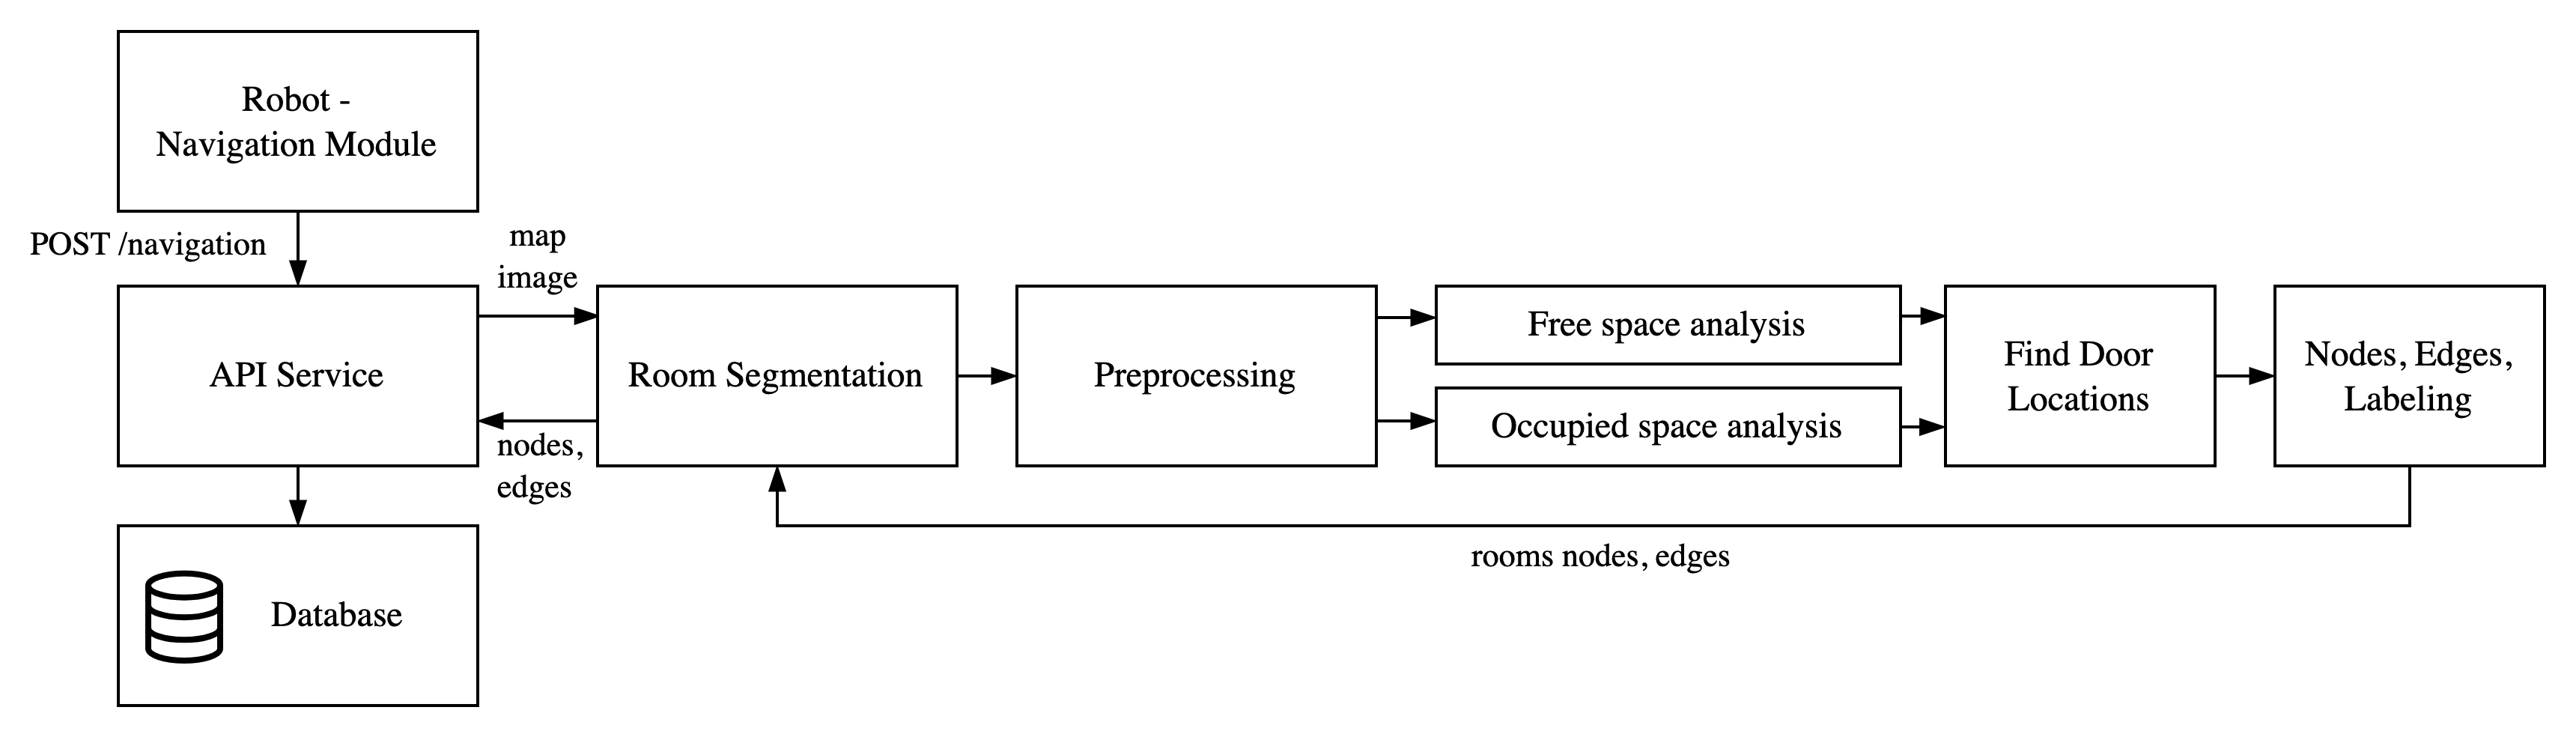
\includegraphics[width=\textwidth]{scene_graph/general_data_flow.png}
  \caption{Schema dei flussi dati per la generazione del grafo di scena e aggiornamento della mappa semantica }
\end{figure}

\section{Generazione del Grafo di Scena}
La generazione del grafo di scena è un passo fondamentale per il mantenimento della coerenza tra Mappa Semantica e Ambiente reale.\\
Il grafo di scena è una struttura dati che rappresenta gli oggetti presenti nell'ambiente e le relazioni tra loro composto da nodi e archi. I nodi rappresentano gli oggetti, mentre gli archi rappresentano le relazioni tra gli oggetti.

\subsection{Lettura del frame RGB-D}

All'interno dell'architettura cloud-native di Robee vi è la presenza di un pod chiamato "Streaming Module" il cui compito è streammare il feed video delle camera sul pod redis del robot, in modo che gli altri servizi o moduli possano accedere a questi dati tramite l'utilizzo di librerie wrapper, rendendo il tutto agnostico rispetto alla tipologia e modello di videocamera montati.

\subsection{Inferenza}
Ogni frame ricevuto dal feed video viene successivamente dato in input al modello PSGTr \cite{yang2022psg} che restituisce un oggetto di tipo Detections il quale contiene i seguenti dati:
\begin{itemize}
  \item labels: lista con lunghezza pari al numero di oggetti rilevati. Ogni valore indica la label corrispondente all' $i$-esimo oggetto. Per esempio, l'oggetto $i$-esimo ha label $labels[i]$;
  \item masks: lista contenente le maschere di ogni oggetto rilevato;
  \item bboxes: lista contenente le bounding boxes di ogni oggetto rilevato;
  \item rel\_pair\_idxes: lista con lunghezza pari al numero di relazioni tra oggetti rilevate. Ogni valore è a sua volta un array di dimensione due dove il primo elemento è l'oggetto target della relazione e il secondo è l'oggetto sorgente della relazione;
  \item rel\_labels: lista con lunghezza pari al numero di relazioni tra oggetti rilevate. Ogni valore indica la label della $i$-esima relazione
  \item rel\_dists: lista con lunghezza pari al numero di relazione tra oggetti rilevate. Ogni valore indica la probabilità associata alla $i$-esima relazione.
\end{itemize}
Questi dati vengono successivamente utilizzati per la costruzione del grafo di scena mediante l'algoritmo seguente.

\subsubsection{Panoptic Scene Graph - Transformer}
Il modello PSGTr \cite{yang2022psg} è un modello di deep learning a singolo stato basato su architettura Transformer \cite{transformer} il cui obiettivo è quello di generare una rappresentazione a grafo della scena data la segmentazione panottica piuttosto che le bounding box degli oggetti rilevati.
\paragraph*{Training}
Il modello, per quanto riguarda gli oggetti, è stato addestrato su un dataset composto da 49mila immagini annotate basato su COCO \cite{coco} e Visual Genome \cite{visualgenemo}. Per le relazioni hanno estratto e costruito un dataset di 56 predicati a partire da dataset come VG-150 \cite{vg150}, VrR-VG \cite{vrvvg} and GQA \cite{cqa}.
\paragraph*{Segmentazione Panoptica}
La segmentazione panoptica individua gli oggetti e assegna a ogni pixel la label della classe dell'oggetto a cui appartengono. L'utilizzo di questa rispetto alle bounding da notevoli vantaggi:
\begin{itemize}
  \item Garantisce una localizzazione più precisa degli oggetti, segmentandoli a livello di pixel e riducendo la presenza di pixel rumorosi o ambigui tipici delle bounding box, che spesso includono porzioni di altre categorie o oggetti;
  \item Copre l'intera scena di un'immagine, inclusi gli sfondi, offrendo una comprensione più completa del contesto rispetto alle bounding box, che tendono a trascurare importanti informazioni di sfondo;
  \item Riduce anche le informazioni ridondanti o irrilevanti presenti nei dataset basati su bounding box, focalizzandosi sulla segmentazione degli oggetti piuttosto che sulle loro parti.
\end{itemize}
\paragraph*{Funzionamento di PSGTr}
Essendo l'architettura di PSGTr basata su DETR \cite{detr} e HOI \cite{hoi}, il modello predice triple $(soggetto, predicato, verbo)$ e la localizzazione degli oggetti simultaneamente.
% TODO: manca la pipeline
\subsection{Costruzione del grafo}
L'algoritmo di costruzione del grafo è costituito da 2 fasi principali:
\begin{itemize}
  \item Costruzione dei nodi per la scena semantica e per la mappa semantica:
  \begin{itemize}
    \item Calcolo della posizione dell'oggetto
  \end{itemize}
  \item Costruzione degli archi per la scena semantica e per la mappa semantica
\end{itemize}

\subsubsection{Costruzione dei nodi}
\paragraph{Estrazione dati dai risultati}
% TODO: Da fare
Estrazione labels, maschere e bounding box dagli mmdections\_results
\paragraph{Calcolo posizioni 3d}
% TODO: Da fare
Prendi la posa delle camere, prendi la terna $x,y,z$ dell'oggetto mascherando il point cloud, applica la matrice camera inversa, get\_tf(posa camera, posizione oggetto dopo camera inversa)


Di seguito è illustrato lo pseudocodice dell'algoritmo in questione.
\begin{algorithm}[H]
  \caption{Costruzione del Grafo di Scena dai risultati dell'inferenza}
  \begin{algorithmic}[1]
  \Procedure{BuildGraph}{$detectionResults, frame$}
  \State $rel\_obj\_labels \gets detectionResults.labels$
  \For{ $l$ in $rel\_obj\_labels$}
    \State $rel\_obj.append(PSG\_CLASSES[l - 1])$
  \EndFor
  \State $rel\_dists \gets mmdet\_results.rel\_dists[:, 1:]$
  \State $rel\_scores \gets \text{max}(rel\_dists, axis=1)$
  
  \State $rel\_top\_idx \gets \text{where}(rel\_scores > \theta)$
  \State $rel\_labels\_topk \gets \text{argmax}(rel\_dists[rel\_top\_idx], axis=1)$
  \State $rel\_pair\_idxes\_topk \gets mmdet\_results.rel\_pair\_idxes[rel\_top\_idx]$
  \State $relations \gets \text{concatenate}([rel\_pair\_idxes\_topk, rel\_labels\_topk])$
  
  \For{$i=0 \text{ to } \text{length}(rel\_obj\_labels)$}\Comment{Costruzione nodi}
      \State $id \gets$ Generate node uuid 
      \State $obj\_map\_position \gets$ Object 3d position map referenced
      \State $obj\_robot\_position \gets$ Object 3d position robot referenced
      \State $node \gets$ Create Node
      \State $camera\_distance \gets distance(obj\_robot\_position - camera\_position)$
      \State $in\_range \gets max\_distance \geq camera\_distance \geq min\_distance$
      \If{$in\_range \text{ and } rel\_obj\_labels[i] \notin bannedLabels$}
          \State $map\_graph.add\_node(node)$
          \If{$camera\_distance \leq frame\_max\_distance$}
            \State $frame\_graph.add\_node(node)$
          \EndIf
      \EndIf
  \EndFor
  
  \For{$r \text{ in } relations$}\Comment{Costruzione archi}
      \State $s\_idx, o\_idx, rel\_id \gets r$
      \State $s\_uuid \gets int\_uuid\_mapping[s\_idx]$
      \State $o\_uuid \gets int\_uuid\_mapping[o\_idx]$
      \If{$map\_graph.get\_node(s\_uuid) \neq \text{None} \text{ and } map\_graph.get\_node(o\_uuid) \neq \text{None}$}
          \For{$obj \text{ in } ["s", "o"]$}
              \State $side \gets \text{locals()}[f"{obj}\_idx"]$
              \State $map\_edge \gets \text{SemanticMapEdge.load}(\{ "source": s\_uuid, "target": o\_uuid, "label": PREDICATES[rel\_id] \})$
              \State $map\_graph.add\_edge(map\_edge)$
              \If{$frame\_graph.get\_node(s\_idx) \neq \text{None} \text{ and } frame\_graph.get\_node(o\_idx) \neq \text{None}$}
                  \State $frame\_edge \gets \text{SemanticMapEdge.load}(\{ "source": str(s\_idx), "target": str(o\_idx), "label": PREDICATES[rel\_id] \})$
                  \State $frame\_graph.add\_edge(frame\_edge)$
              \EndIf
          \EndFor
      \EndIf
  \EndFor
  
  \Return $map\_graph, frame\_graph$
  \EndProcedure
  \end{algorithmic}
  \end{algorithm}

\subsubsection{Costruzione degli archi}

\section{Aggiormento del Mappa Semantica}
\subsection{Stanza corrente robot}
\subsection{Proiezione del Camera Frustum}
\subsection{Controllo della posizione degli oggetti}
\subsection{Aggiornamento e salvataggio a DB}



\section{Conclusioni}

